%%%%%%%%%%%%%%%%%%%%%%%%%%%%%%%%%%%%%%%%%%%%%%%%%%%%%%%%%%%%%%%%%%%%%%%%%%%%%%%%
% Inicializálás                                                                %
%%%%%%%%%%%%%%%%%%%%%%%%%%%%%%%%%%%%%%%%%%%%%%%%%%%%%%%%%%%%%%%%%%%%%%%%%%%%%%%%

%%%%%%%%%%%%%%%%%%%%%%%%%%%%%%%%%%%%%%%%%%%%%%%%%%%%%%%%%%%%%%%%%%%%%%%%%%%%%%%%
% Papírméret, betűméret, margó, magyar karakterek                              %
%%%%%%%%%%%%%%%%%%%%%%%%%%%%%%%%%%%%%%%%%%%%%%%%%%%%%%%%%%%%%%%%%%%%%%%%%%%%%%%%

\documentclass[a4paper,12pt]{article}
\special{papersize=210mm,297mm}

\usepackage{anysize}
\marginsize{2.5cm}{2.5cm}{2.5cm}{2.5cm}

\usepackage[utf8]{inputenc}
\usepackage[magyar]{babel}

%%%%%%%%%%%%%%%%%%%%%%%%%%%%%%%%%%%%%%%%%%%%%%%%%%%%%%%%%%%%%%%%%%%%%%%%%%%%%%%%
% Fedlap inicializálása                                                        %
%%%%%%%%%%%%%%%%%%%%%%%%%%%%%%%%%%%%%%%%%%%%%%%%%%%%%%%%%%%%%%%%%%%%%%%%%%%%%%%%

\usepackage{fedlap}

\csapat{unexpected\_exceptions}{59}
\konzulens{Ferencz Endre}

\taga{Biró Loránd}{NCZAGL}{lol.kylerrr@gmail.com}
\tagb{Kanyó Tibor}{NXWUKE}{kanyo.tibi@gmail.com}
\tagc{Magyar Dániel}{SUFFGT}{samuraidanm@gmail.com}
\tagd{Tarjáni Tamás}{S499KV}{tarjanitomi@gmail.com}
\tage{Vajsz Kornél}{VUYNAW}{roncsipar@gmail.com}

%%%%%%%%%%%%%%%%%%%%%%%%%%%%%%%%%%%%%%%%%%%%%%%%%%%%%%%%%%%%%%%%%%%%%%%%%%%%%%%%
% Fejléc és lábléc                                                             %
%%%%%%%%%%%%%%%%%%%%%%%%%%%%%%%%%%%%%%%%%%%%%%%%%%%%%%%%%%%%%%%%%%%%%%%%%%%%%%%%

\usepackage{fancyhdr}

\setlength{\headheight}{1.4em}
\setlength{\headsep}{2em}

\fancyhf{}
\fancyhead[OL] { \leftmark{} }
\fancyhead[OR] { \tmpcsapat }
\fancyfoot[OC] { \thepage }
\fancyfoot[OR] { \tmpdatum }

\pagestyle{fancy}

%%%%%%%%%%%%%%%%%%%%%%%%%%%%%%%%%%%%%%%%%%%%%%%%%%%%%%%%%%%%%%%%%%%%%%%%%%%%%%%%
% Napló                                                                        %
%%%%%%%%%%%%%%%%%%%%%%%%%%%%%%%%%%%%%%%%%%%%%%%%%%%%%%%%%%%%%%%%%%%%%%%%%%%%%%%%

\usepackage{longtable}

\newenvironment{journal}
{
	\hbadness 10000
	\begin{longtable}{|p{60pt}|l|l|p{216pt}|}
	\hline
	\textbf{Kezdet} & \textbf{Időtartam} & \textbf{Résztvevők} & \textbf{Leírás} \\
	\hline
	\endfirsthead
	\hline
	\textbf{Kezdet} & \textbf{Időtartam} & \textbf{Résztvevők} & \textbf{Leírás} \\
	\hline
	\endhead
}
{
	\end{longtable}
}

\newcommand{\journalentry}[4]
{
	{#1} & {#2} óra & \parbox{50pt}{#3} & {#4} \\
	\hline
}

%%%%%%%%%%%%%%%%%%%%%%%%%%%%%%%%%%%%%%%%%%%%%%%%%%%%%%%%%%%%%%%%%%%%%%%%%%%%%%%%
% UseCase leírás                                                               %
%%%%%%%%%%%%%%%%%%%%%%%%%%%%%%%%%%%%%%%%%%%%%%%%%%%%%%%%%%%%%%%%%%%%%%%%%%%%%%%%

\newenvironment{usecase}
{
	\hbadness 10000
	\begin{longtable}[l]{|p{100pt}|p{328pt}|}
	\hline
	\endfirsthead
	\hline
	\endhead
}
{
	\hline
	\end{longtable}
}

\newcommand{\usecaseentry}[2]
{
	\hline
	\textbf{#1} & {#2}\\
}

%%%%%%%%%%%%%%%%%%%%%%%%%%%%%%%%%%%%%%%%%%%%%%%%%%%%%%%%%%%%%%%%%%%%%%%%%%%%%%%%
% FileList leírás                                                               %
%%%%%%%%%%%%%%%%%%%%%%%%%%%%%%%%%%%%%%%%%%%%%%%%%%%%%%%%%%%%%%%%%%%%%%%%%%%%%%%%

\newenvironment{filelist}
{
	\hbadness 10000

	\begin{longtable}{|p{145pt}|p{35pt}|p{63pt}|p{163pt}|}
	\hline
	\textbf{Fájl neve} & \textbf{Méret} & \textbf{Keletkezés ideje} & \textbf{Tartalom} \\
	\hline
	\endfirsthead
	\hline
	\textbf{Fájl neve} & \textbf{Méret} & \textbf{Keletkezés ideje} & \textbf{Tartalom} \\
	\hline
	\endhead
}
{
	\end{longtable}
}

\newcommand{\filelistentry}[4]
{
	{#1} & {#2} b & {#3} & {#4} \\
	\hline
}
%%%%%%%%%%%%%%%%%%%%%%%%%%%%%%%%%%%%%%%%%%%%%%%%%%%%%%%%%%%%%%%%%%%%%%%%%%%%%%%%
% Egyebek                                                                      %
%%%%%%%%%%%%%%%%%%%%%%%%%%%%%%%%%%%%%%%%%%%%%%%%%%%%%%%%%%%%%%%%%%%%%%%%%%%%%%%%

\usepackage{graphicx}		% Kepek beillesztesehez
\usepackage{epstopdf}		% EPS fajlok felismeresehez
\graphicspath{{Images/}}	% Az Images mappaban keresse a kepeket

\anyag{7. Prototípus koncepciója}
\datum{2012. március 25.}
\setcounter{section}{6}

%%%%%%%%%%%%%%%%%%%%%%%%%%%%%%%%%%%%%%%%%%%%%%%%%%%%%%%%%%%%%%%%%%%%%%%%%%%%%%%%
% Dokumentum                                                                   %
%%%%%%%%%%%%%%%%%%%%%%%%%%%%%%%%%%%%%%%%%%%%%%%%%%%%%%%%%%%%%%%%%%%%%%%%%%%%%%%%

\begin{document}

\fedlap

\section{Prototípus koncepciója}

\subsection{Prototípus interface-definíciója}

\subsubsection{Az interfész általános leírása}
A standard bemenet és kimenet adta lehetőségekből adódóan, a program indításakor módunk van betölteni kész storyboardot az \emph{\textless  utvonal\textbackslash tesztpalya.xml} argumentummal. Továbbá a kimenetet is rögvest írathatjuk fájlba, ha a standard kimenetet átírányítjuk a \emph{\textgreater  utvonal\textbackslash kimenet.txt} kapcsolóval.
A program bemenete néhány vezérlőparancs, melyek megfeleltethető a játék irányítását szabályozó külső és belső vezérlőknek: játékos és pályaelemek mozgatása, és a szimuláció futtatása.

\subsubsection{Bemeneti nyelv}

%\begin{usecase}
%	\usecaseentry{Parancs neve}{Indítási argumentumok}
%	\usecaseentry{Rövid leírás}{Az alkalmazás indításakor megadhatunk bemeneti paraméterek, ezzel is változtatva részletekben az alkalmazás működését.}
%	\usecaseentry{Opciók}{
%	\begin{description}
%	\item[- -resolution vagy -r]: a felbontást adhatjuk meg vele, egy nem negatív egész számot vár
%	\item[- -animate vagy -a]: beállíthatjuk, hogy legyenek-e animálva a játékban történő változások képi megjelenései,
%	\item[- -silent vagy -s]: kikapcsolható az összes kimenet , mely a renderelés során történik
%	\item[- -help vagy -h vagy help]: kilistázza az összes lehetséges parancsot
%	\end{description}}
%\end{usecase}

\begin{usecase}
	\usecaseentry{Parancs neve}{px \textless movetype\textgreater}
	\usecaseentry{Rövid leírás}{Ez az általános szintaxisa a játékosok mozgatásának.}
	\usecaseentry{Opciók}{
	\begin{description}
		\item[px]: lehet p1 vagy p1, attól függően, hogy kit szeretnénk mozgatni
		\item[\textless movetype\textgreater]: a mozgás irányát állíthatjuk vele, lehetséges értékei: left, right,stop,jump
	\end{description}}
\end{usecase}

\begin{usecase}
	\usecaseentry{Parancs neve}{slide \textless direction\textgreater}
	\usecaseentry{Rövid leírás}{Ezen paranccsal egy pályaelemet mozgathatunk az üres helyre.}
	\usecaseentry{Opciók}{\textbf{\textless direction\textgreater}: melyik irányba mozgassuk a pályaelemet, lehetséges értékei: up,down,left,right}
\end{usecase}

\begin{usecase}
	\usecaseentry{Parancs neve}{go \textless frames\textgreater}
	\usecaseentry{Rövid leírás}{A következő \textless frames\textgreater mennyiségű kép szimulációjának indítása}
	\usecaseentry{Opciók}{\textbf{\textless frames\textgreater}: hány képkockát szimuláljunk előre}
\end{usecase}

\subsubsection{Kimeneti nyelv}

A parancsok kimenete egyértelműen leolvasható a karakteres felületről. A pályaelemek mozgatását követően kiírásra kerül az új pályaelrendezés. A játékos mozgatását végző parancsok kimenete nem látszik azonnal, ehhez előbb meg kell adni, hogy milyen időre szeretnénk szimulálni. A szimuláció hatására kikerül a konzolra mindkét játékos minden képkockára vett pozíciója valamint az, hogy mi a pálya állapota, a megadott képkockák szimulálása után pedig megjelenítésre kerül a pálya.

\newpage

A 0 kezdetű számozásnál a 2. képkocka során leolvasható a játékosok pozíciója (pl. az első játékos a [0, 1] koordinátájú LevelPart-ban van, és a pozíciója azon belül [1,50, 7,50]), és hogy a pályát még nem teljesítettük és a kulcsokat még fel kell szednünk hozzá:
\begin{verbatim}
	2 P1[1, 0][1,50, 7,50] P2[1, 0][0,50, 7,50] {Normal}
\end{verbatim}

Pálya megjelenítése az alábbi mintára épül. A pályán D az ajtót, K a kulcsot, a számok a két játékost, a függőleges és vízszintes vonalak az adott pályaelem széleit illetve az X a blokkokat jelöli.
%Előfordulhat, hogy a játékosok több szomszédos mezőben is egyidejűleg megjelennek a konzolon, amennyiben olyan a másodpercenkénti képkockák száma, hogy a szimulációs során a játékos kiterjedése több mezőben helyezkedik el. Ekkor tehát az egyes mezők határain van, így a rendszer szerint jogosan mindegyik helyen ott van.

\begin{verbatim}
------------------------
|XXX  XXXXX||          |
|          ||          |
|          ||          |
|          ||          |
|          ||          |
|          ||    K     |
|          ||   XX     |
|      D  K||21 XXXX   |
|XXXXXXXXXX||XXXXXXXXXX|
|XXXXXXXXXX||XXXXXXXXXX|
------------------------
            ------------
            |          |
            |          |
            |          |
            |          |
            |          |
            |          |
            |          |
            | K        |
            |XXX  XXXXX|
            |XXX  XXXXX|
            ------------
\end{verbatim}


\subsection{Összes részletes use-case}
Amely use-case leírásánál nem szerepel az \textbf{Aktorok} rész, annál a \textbf{Player} az aktor. Az alábbi leírásoknál külön nincs feltüntetve a \textbf{Forgatókönyv} rész, mivel folytonos időben történik a játék működése, azaz a virtuális világban igen apró lépésközökkel történik az állapotot változásának számítása, így túl aprólékos és részletes lenne mindegyik forgatókönyv kifejtése. Ezeket az \textbf{5.4 fejezet Szekvencia diagramok a belső működésre} című részében mutattuk meg folyamatukban.

\begin{center}
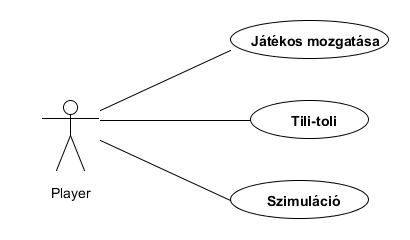
\includegraphics[scale=0.65]{07_UseCase.png}
\end{center}

\begin{usecase}
	\usecaseentry{Use-case neve}{Játékos mozgatása}
	\usecaseentry{Rövid leírás}{A kettő közül valamelyik emberkét (a programban a játékos száma szimbolizálja) tudjuk irányítani. Meghatározhatjuk, hogy melyiküket utasítjuk, illetve hogy jobbra vagy balra menjen, ugorjon, esetleg álljon meg.}
\end{usecase}
\begin{usecase}
	\usecaseentry{Use-case neve}{Tili-toli}
	\usecaseentry{Rövid leírás}{A játék tili-toli módja, amikor pályaelemeket mozgathatunk.}
\end{usecase}
\begin{usecase}
	\usecaseentry{Use-case neve}{Szimuláció}
	\usecaseentry{Rövid leírás}{A nem pillanatszerű történések (pl. a játékosok mozgása) folyamatos időben történnek, de a konzolos megjelenítés sajátosságai miatt ebből csak egyes pillanatokat tudunk kiragadni. Ehhez időről időre szimulálnunk kell a világ változását a következő megjelenített időpillanatig.}
\end{usecase}

\subsection{Tesztelési terv}
A bemeneti fájlban azon parancsok egy szekvenciáját adhatjuk meg, amiket egyébként is megadhatnánk a program futása közben (px, slide, go), ezáltal egyszerűbbé válik a tesztelés, mivel az ilyen "forgatókönyvek" futtatása abszolút determinisztikus és így minden felfedezett hiba tökéletesen reprodukálható. Természetesen lehetőség van a parancsok egyenkénti konzolba gépelésével is irányítani a játékot. A kimenetet szintén választhatjuk akár egy szövegfájlnak, akár a konzolképernyőnek. A kimeneten megfigyelhető változások minden esetben összhangban vannak a bevitt parancsokkal, idő- és sorrendhelyesen következnek belőlük. Mindez a kimeneten egyszerűen követhető, mivel a pálya egyes állapotai szépen kirajzolódnak.

\newpage

\begin{usecase}
	\usecaseentry{Test-eset neve}{01 Játékos irányítása \#1}
	\usecaseentry{Rövid leírás}{A két játékos egy 1x1 pályarészből álló pályán van amikben több össze-vissza elhelyezett téglalap alakú blokk található. A két játékos minden irányban ugrál és mozog.}
	\usecaseentry{Teszt célja}{Ezzel a teszttel megfigyelhető hogy a játékosok egyszerű mozgatása és az ütközésvizsgálat a téglalap alakú blokkokkal a várt módon történnek.}
\end{usecase}

\begin{usecase}
	\usecaseentry{Test-eset neve}{02 Játékos irányítása \#2}
	\usecaseentry{Rövid leírás}{A két játékos ugyancsak egy 1x1 pályarészből álló pályán van amikben több össze-vissza elhelyezett téglalap és háromszög alakú blokk is található. A két játékos minden irányban ugrál és mozog.}
	\usecaseentry{Teszt célja}{Ezzel a teszttel megfigyelhető hogy a játékosok egyszerű mozgatása és az ütközésvizsgálat a háromszög alakú blokkokkal a várt módon történnek.}
\end{usecase}

\begin{usecase}
	\usecaseentry{Test-eset neve}{03 Kulcsok és ajtó}
	\usecaseentry{Rövid leírás}{A két játékos továbbra is egy 1x1 pályarészből álló pályán van amikben 3 kulcs van elhelyezve. A két játékos sorra felveszik a kulcsokat, de minden kulcs felvétele előtt legalább az egyik átmegy az ajtó előtt. Végül a 3. kulcs felvétele után az egyik játékos az ajtóhoz megy és a pálya befejeződik.}
	\usecaseentry{Teszt célja}{Ezzel a teszttel megfigyelhető hogy a kulcsok felvételének kezelése és az ajtóval való ütközés vizsgálata a várt módon működik.}
\end{usecase}

\begin{usecase}
	\usecaseentry{Test-eset neve}{04 Pályarész határok}
	\usecaseentry{Rövid leírás}{Egy egyszerű 2x2-1 pályarészből álló pályán való egyszerű mozgást tesztelünk. Miközben a pályarészeket néha-néha elcsúsztatjuk a játékosokkal legalább egyszer áthaladunk valamely pályarész határán majd később valamikor megakadunk egy másikon. A teszt során mindkét játékos egyszer "szakadékba" zuhan és visszakerül a kezdő pozíciójára, majd ezután úgy sétálnak bele a lyukba hogy van alatta illeszkedő pályarész, és sikeresen átkerülnek rá. }
	\usecaseentry{Teszt célja}{Ez a teszt bemutatja hogy a pályarészek csúsztatása, a határokon való áthaladás és a "halál" vagyis a kezdőpontra visszahelyezés jól működik.}
\end{usecase}

\newpage

\begin{usecase}
	\usecaseentry{Test-eset neve}{05 Főpróba}
	\usecaseentry{Rövid leírás}{Egy pálya végigvitelét láthatjuk, az elejétől a végéig. A két játékos mozog, egy pályaelemet mozgatunk, a játékosok átmennek az előbb mozgatott pályaelembe, az egyikük (1-es) leesik egy olyan szakadékba, amelynek nincs másik pályaelemben folytatása és meghal. Ekkor a kezdőhelyén éled újra, és ismét elindul az előző útján, eközben mozgatunk egy pályaelemet és a 2-es számú játékos leesik az immár a helyén lévő végső pályaelembe. Itt felveszi az utolsó kulcsot, majd végül az 1-es játékos az ajtóhoz megy és vége a pályának.}
	\usecaseentry{Teszt célja}{A program általános működésének bemutatása: játékosok és pályaelemek mozgatása, halál, kulcsok felvétele, illetve kooperatív módú győzelem.}
\end{usecase}

\subsection{Tesztelést támogató segéd- és fordítóprogramok specifikálása}
A fordítóprogram és annak működési szabálya megegyezik a 6.1.2 Fordítás nevű fejezetben leírtakkal. A \emph{build.bat} fájlt futtatva a konzolból, előáll a a lefordított jar fájl. A fájl az alábbi utasításokat tartalmazza, melyben csak jar neve változott:

\begin{verbatim}
@echo off
if not exist bin (mkdir bin)

echo Compiling classes...
javac src/main/*.java src/model/*.java src/gameLogic/*.java -d bin
        -encoding UTF-8

cd bin
echo Creating jar...
jar cfm ../ContinuityPrototype.jar ../src/manifest.txt main/*.class
        model/*.class gameLogic/*.class
cd ..

echo Done
@echo on
\end{verbatim}

A tesztelés megkönnyítése érdekében, létrehoztunk egy batch fájlt: \emph{run.bat}. Ezen fájlt kell futtatni a főkönyvtárból. A fájl maximum négy darab értéket vár indítási paraméternek, ezek választható értékei a \emph{Bemeneti nyelv} fejezet \emph{Indítási argumentumok} nevű részben vannak kifejtve. Ezen fájl az alábbi parancsot végrehajtva elindítja az elkészült jar fájlt: 
\begin{verbatim}
@echo off
java -jar ContinuityPrototype.jar %1 %2 %3 %4
@echo on
\end{verbatim}


\subsection{Napló}

\begin{journal}
\journalentry{2012.03.21. 13:30}{1.5}{Biró, Kanyó, Magyar, Tarjáni, Vajsz}{Értekezlet, lefektettük a prototípus koncepcióját.}
\journalentry{2012.03.23. 8:00}{1}{Kanyó}{Dokumentum sablon elkészítése. Tesztelési segéd- és fordítóprogramok leírása. Bemeneti parancsok leírása}
\journalentry{2012.03.23. 19:30}{1}{Kanyó}{Hibák felkutatása a kód működésében. Parancsok leírásának korrigálása. Kimeneti nyelv definiálása.}
\journalentry{2012.03.24. 22:00}{1}{Biró}{Tesztesetek kidolgozása, leírása}
\journalentry{2012.03.24. 22:00}{2}{Tarjáni}{Use-case fejezet, teszteset bevezető, tesztesetek leírása.}
\end{journal}

\end{document}